
\chapter{Mise en \oe{}uvre de \PpFf}
\label{implementation.chap}


\begin{figure}
\centering
     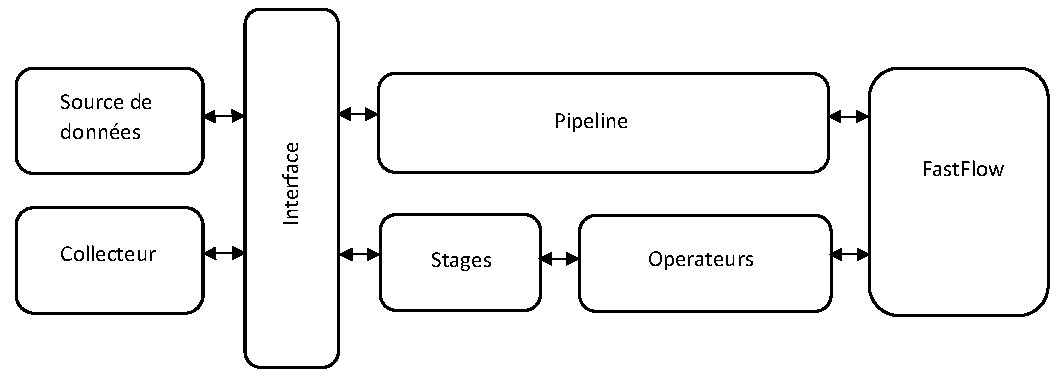
\includegraphics[width=1.0\textwidth]{Figures/AllComponentsAPI.pdf}
      \caption{Les composants de \TT{PpFf}.}
       \label{AllComponentsAPI.fig}
\end{figure}


Ce chapitre pr\'esente une description d\'etaill\'ee de la fa\c{c}on dont \TT{PpFf} est impl\'ement\'e. Une vue d'ensemble des composants de \TT{PpFff} est pr\'esent\'ee \`a la figure~\ref{AllComponentsAPI.fig}. De fa\c{c}on g\'en\'erale, la mise en \oe{}uvre est bas\'ee sur la biblioth\`eque \TT{FastFlow}, h\'eritant et \'etendant plusieurs de ses classes. La premi\`ere section montre les couches de l'API et les liens entre elles.  La deuxi\`eme section d\'ecrit comment le pipeline du flux est mis en œuvre. La section suivante examine comment la parall\'elisation du flux est r\'ealis\'ee. Les \emph{stages} sont d\'ecrits dans la quatri\`eme section. La cinqui\`eme section pr\'esente la description d'un exemple complet d\'ecrivant comment un programme \PpFf{} est compil\'e et ex\'ecut\'e. Le chapitre se termine en pr\'esentant quelques donn\'ees sur le code de cette mise en \oe{}uvre.
%
\GT{Ajouter ici une remarque sur (et une référence à) l'annexe qui
décrit quelques donn\'ees sur la mise en \oe{}uvre}

\section{Mise en \oe{}uvre multi-couches de \PpFf{} via \TT{FastFlow}}


\begin{figure}
\centering
     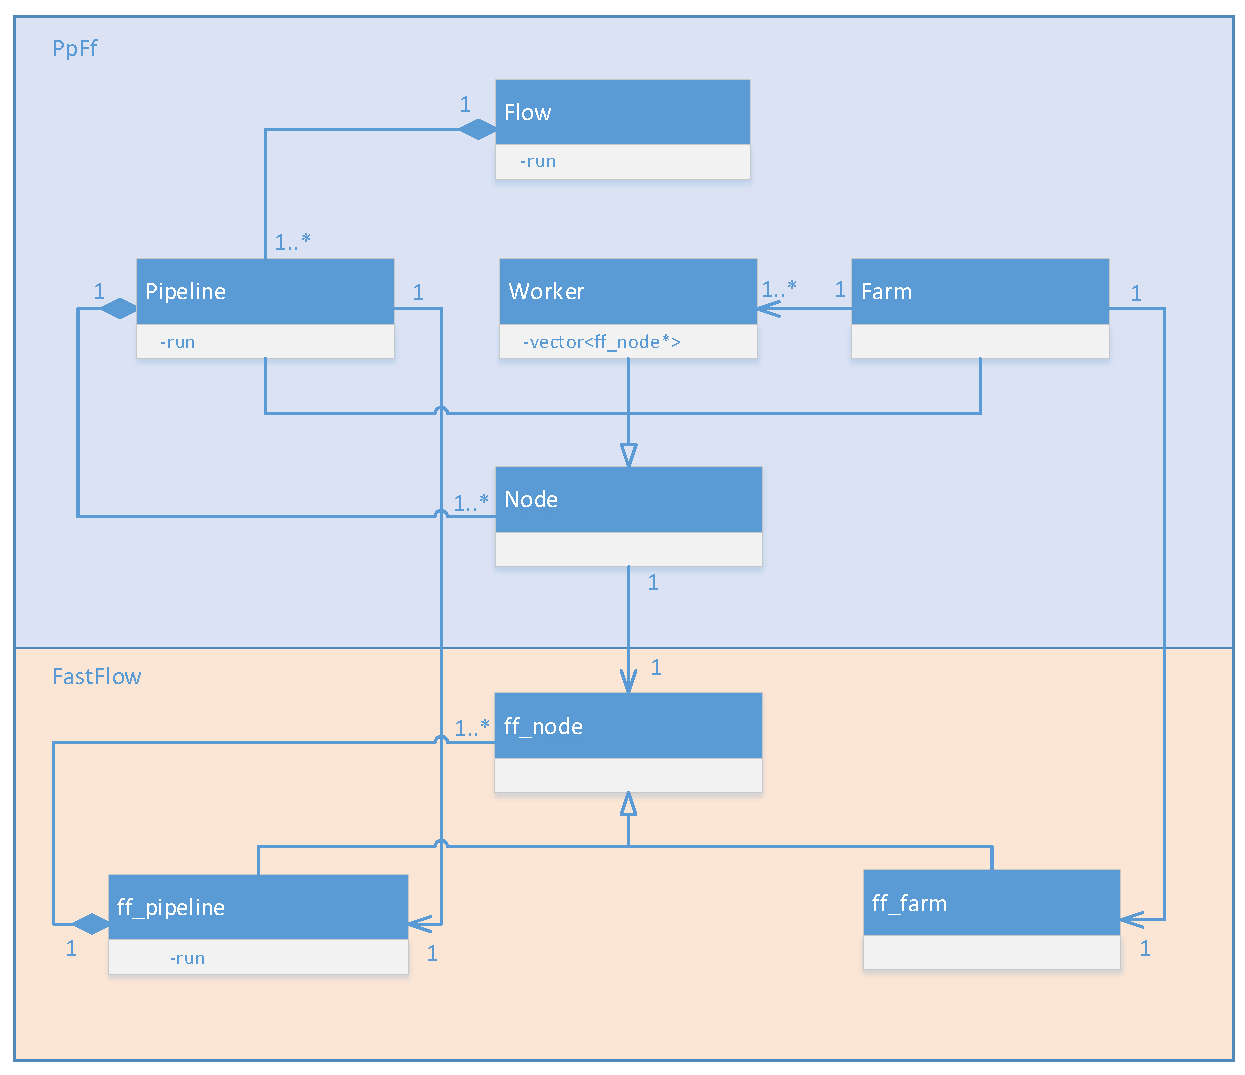
\includegraphics[width=1.0\textwidth]{Figures/CorrespondencePpFfToFastFlow.pdf}
      \caption{La correspondance entre les \'el\'ements de \TT{PpFf} et ceux de  \TT{FastFlow}.}
       \label{CorrespondencePpFfToFastFlow.fig}
\end{figure}


%\begin{figure}
%\centering
%     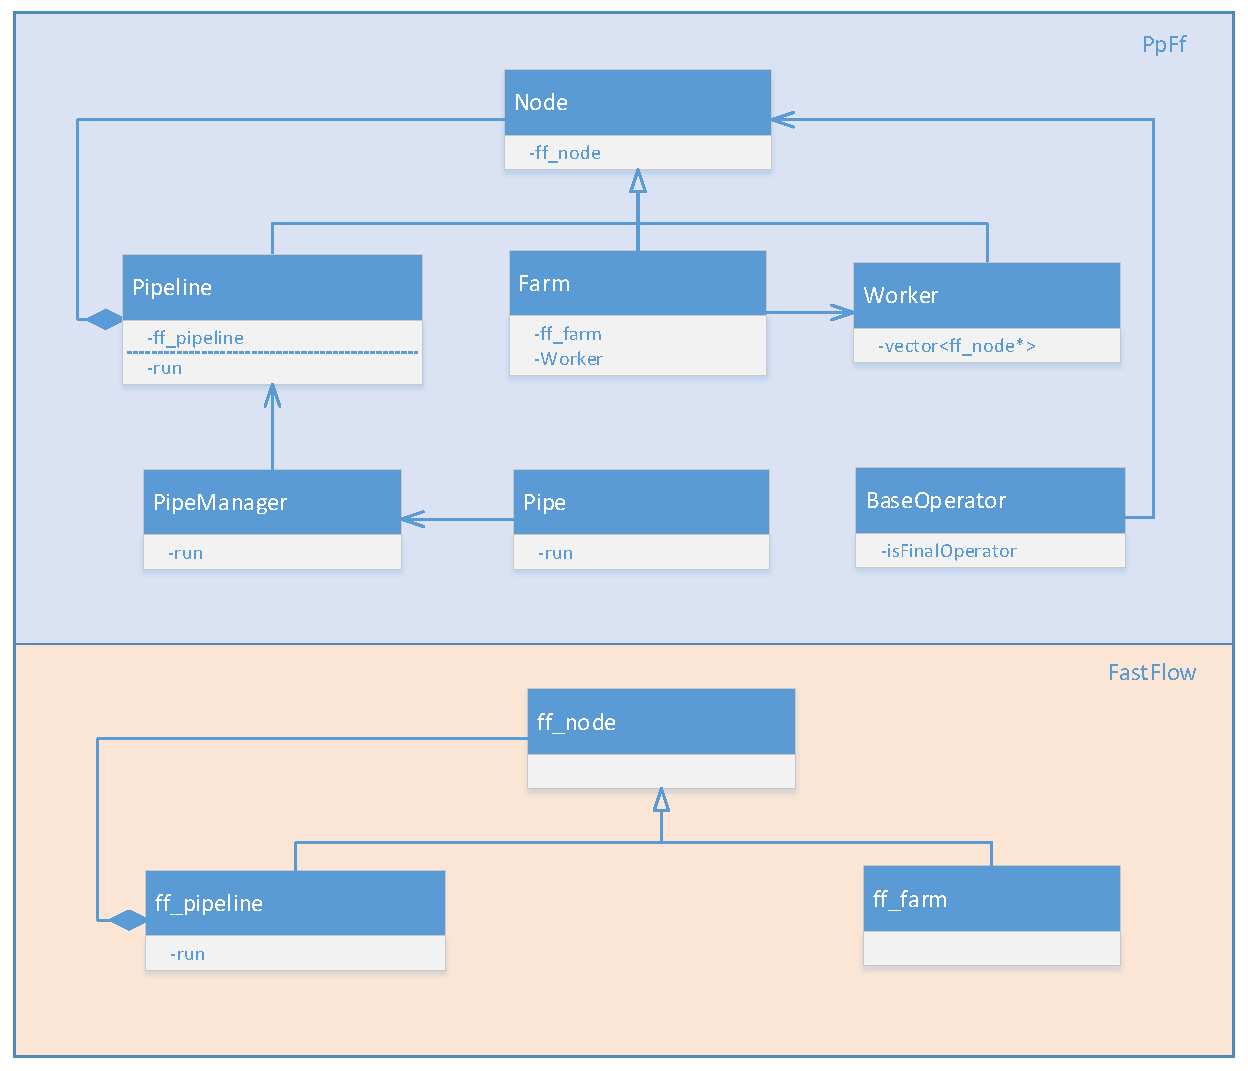
\includegraphics[width=1.0\textwidth]{Figures/MapToFastFlow.pdf}
%      \caption{La correspondance entre les \'el\'ements de \TT{PpFf} et ceux de  \TT{FastFlow}.}
%       \label{MapToFastFlow.fig}
%\end{figure}


\ppff{} est impl\'ement\'e au--dessus de la biblioth\`eque \TT{FastFlow}, de sorte que nous utilisons les constructions \TT{ff\_node}, \TT{ff\_pipeline} et \TT{ff\_farm} de \TT{FastFlow}. La figure~\ref{CorrespondencePpFfToFastFlow.fig} montre la correspondance entre les \'el\'ements de \TT{PpFf} et ceux de \TT{FastFlow}. Chaque classe susmentionn\'ee de \TT{FastFlow} a une association dans \TT{PpFf}. Par exemple, l'impl\'ementation de la classe \TT{Node} de \TT{PpFf} est r\'ealis\'ee par l'entremise de la classe \TT{ff\_node} de \TT{FastFlow}. Ce m\'ecanisme a permis d'ajouter plus de fonctionnalit\'es \`a l'API tout en b\'en\'eficiant des performances offertes par \TT{FastFlow}.



\section{Mise en \oe{}uvre des pipelines}

Un pipeline, un objet de classe \TT{Pipeline}, repr\'esente une cha\^ine de traitement. Un \TT{Pipeline} est compos\'e par une s\'erie d'op\'erations sp\'ecifi\'ees par l'utilisateur qui sont appliqu\'ees aux \'el\'ements d'un flux. Comme on peut le voir dans la figure~\ref{CorrespondencePpFfToFastFlow.fig}, un \TT{Pipeline} utilise les fonctionnalit\'es de la classe \TT{ff\_pipeline} de \TT{FastFlow}. 

Celles qui composent un \TT{Pipeline} sont de deux types : les op\'erations sans \'etat et avec \'etat. Un \TT{Pipeline} contient une ou plusieurs op\'erations sans \'etat et une seule op\'eration avec \'etat. Lorsque cette derni\`ere est ajout\'ee dans le \TT{Pipeline}, la m\'ethode \TT{run()} du \TT{Pipeline} est appel\'ee. \`A ce stade, un objet de type \TT{ff\_pipeline} correspondant au \TT{Pipeline} est cr\'e\'e. Ensuite, chaque op\'eration sp\'ecifi\'ee par l'utilisateur est visit\'ee et, en fonction de la configuration \'etablie, des objets de type \TT{ff\_node} ou \TT{ff\_farm} sont ajout\'es dans l'objet \TT{ff\_pipeline}. Chaque nœud ainsi ajout\'e dans \TT{ff\_pipeline} sera alors ex\'ecut\'e dans un fil d'ex\'ecution ind\'ependant (\emph{thread}), une caract\'eristique de la mise en \oe{}uvre de \TT{FastFlow}.
%La cr\'eation d'un \TT{Pipeline} est r\'ealis\'ee \`a l'aide de la classe \TT{PipeManager}, dont les d\'etails sont omis.


\section{\'Ex\'ecution parall\`ele avec parall\'elisme de flux ou de donn\'ees}

La cr\'eation de code parall\`ele est g\'en\'eralement consid\'er\'ee du domaine d'experts. La complexit\'e de l'\'ecriture de code parall\`ele diminue la productivit\'e, ce qui peut augmenter les co\^uts de d\'eveloppement. Par contre, \TT{PpFf} permet aux programmeurs de composer des morceaux de code s\'equentiel --- des fonctions ou expressions lambdas --- et d'ex\'ecuter le tout en parall\`ele. Par l'interm\'ediaire d'une interface unique, l'API offre deux mod\`eles de parall\'elisme : le parall\'elisme de flux et le parall\'elisme de donn\'ees.



\subsection{Parall\'elisme de flux}

Le parall\'elisme de flux consiste \`a ex\'ecuter plusieurs \'etapes d'un traitement s\'equentiel en parall\`ele en leur faisant traiter des donn\'ees diff\'erentes. Les donn\'ees se succ\`edent ainsi les unes aux autres dans les diff\'erentes \'etapes --- appel\'ees  aussi des \emph{stages} (cf.~Section~\ref{stages.sect}).
%
Le traitement effectu\'e dans un \emph{stage} \`a un instant donn\'e peut d\'ependre, ou non, des traitements effectu\'es par ce m\^eme \emph{stage} pour les donn\'ees pr\'ec\'edentes --- un \'etat interne peut donc \^etre conserv\'e. 
%
\`A noter que ce type de parall\'elisme est appliqu\'e par d\'efaut dans notre API. 
%
Ce fonctionnement permet de parall\'eliser des traitements avec des d\'ependances entre les donn\'ees sans avoir recours \`a des synchronisations \emph{explicites} par le programmeur. 

\goodbreak
\begin{samepage}
Un flux compos\'e de $n$ \emph{stages} $S_1, S_2, \ldots, S_n$ o\`u le \emph{stage} $S_i$ ex\'ecute une op\'eration $O_i$ peut \^etre exprim\'e sous la forme d'une composition s\'equentielle d'op\'erations sur les \'el\'ements d'entr\'ee comme suit, o\`u $O(x)$ repr\'esente le traitement global d'un \'el\'ement $x$ du flux~: 
%
\[
	O(x) = O_n( \ldots (O_k( \ldots O_1(x)) \ldots ) \ldots ));
\]
\end{samepage}


\begin{figure}
\centering
     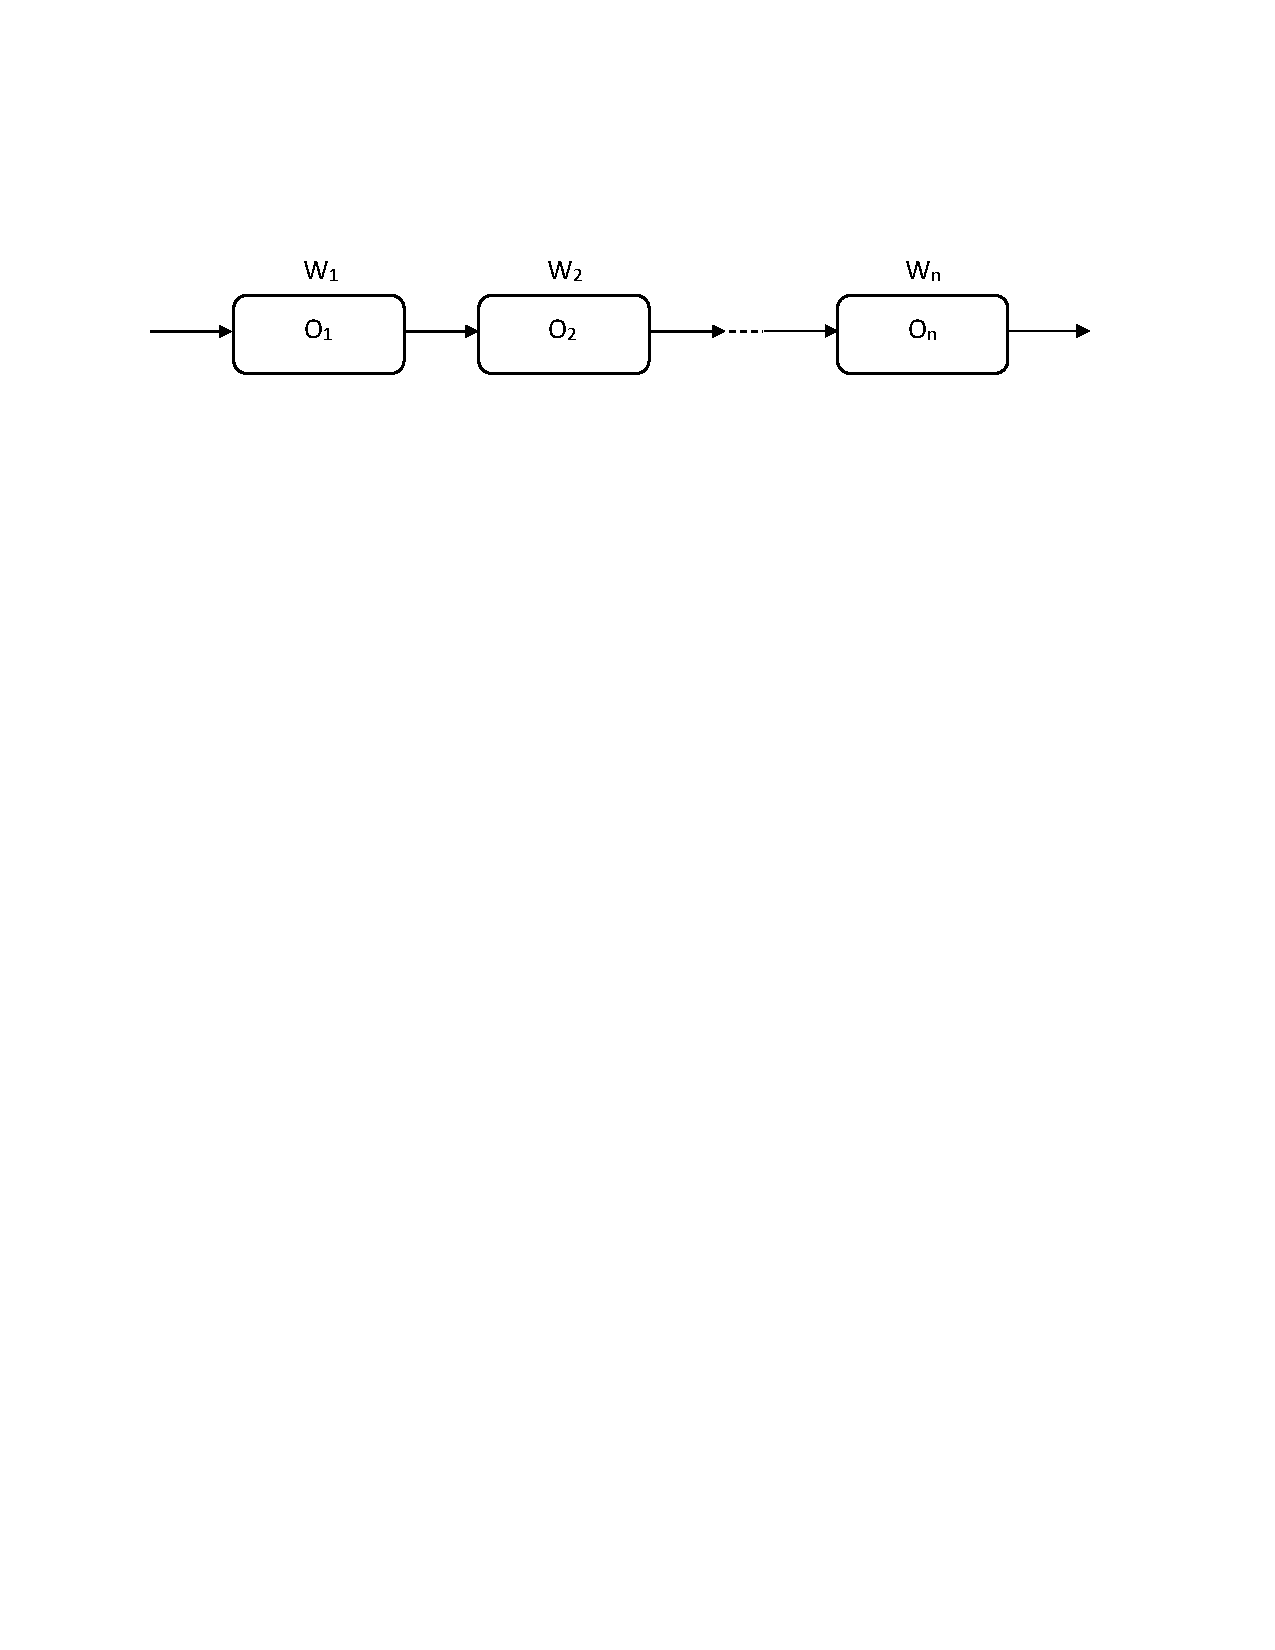
\includegraphics[width=1.0\textwidth]{Figures/ParallelismeDuFlux.pdf}
      \caption[Une repr\'esentation graphique du parall\'elisme de flux en \ppff.]{Une repr\'esentation graphique du parall\'elisme de flux pour une d\'ecomposition en $n$ \emph{stages} $S_1, S_2, \ldots, S_n$. Les op\'erations $O_1, O_2, \ldots, O_n$ sont ex\'ecut\'ees de fa\c{c}on parall\`ele dans diff\'erents fils d'ex\'ecution $W_1, W_2, \ldots, W_n$ ($W$ pour \emph{$W$orker}).}
       \label{ParallelismeDuFlux.fig}
\end{figure}


Si on note par $W_i$ le fil d'ex\'ecution (\emph{thread}) associ\'e au \emph{stage} $S_i$, alors
le parall\'elisme de flux du pipeline peut \^etre repr\'esent\'e par un graphe lin\'eaire de $n$ travailleurs. Chaque travailleur correspond \`a une op\'eration sp\'ecifique $O_i$. La figure~\ref{ParallelismeDuFlux.fig} montre la repr\'esentation graphique du parall\'elisme de flux dans un tel pipeline. Signalons que cette solution n'acc\'el\`ere pas le calcul d'un seul \'el\'ement; par contre, elle am\'eliore \emph{le d\'ebit de sortie}.

\subsection{Parall\'elisme de donn\'ees}

Le parall\'elisme de donn\'ees impl\'ement\'e dans \TT{PpFf}  consiste \`a r\'epliquer une op\'eration sur un ensemble de travailleurs identiques. Autrement dit, il vise \`a effectuer un traitement identique sur un ensemble de donn\'ees ind\'ependantes les unes des autres. 
%
Dans notre impl\'ementation de \PpFf, le parall\'elisme de donn\'ees est mis en \oe{}uvre avec les \emph{Task Farm} de \TT{FastFlow}.


D\'ecrit \`a la section~\ref{farm.sect}, un \emph{Task Farm} est compos\'ee de trois entit\'es : un \emph{Emitter}, plusieurs instances de travailleurs (\emph{workers}) et un \emph{Collector}. Par d\'efaut, dans \PpFf{}, les \'el\'ements sont r\'epartis par un \emph{Emitter} aux divers travailleurs selon une politique \emph{round robin}.%
%
\footnote{Politique \emph{round robin}~: approche d'ordonnancement pour r\'epartir la charge du travail entre des \emph{threads}, avec une file d'attente circulaire. Cf.~\url{https://fr.wikipedia.org/wiki/Round-robin_(informatique)}.} 
%
Les travailleurs re\c{c}oivent les \'el\'ements d'entr\'ee et appliquent sur chacun l'op\'eration sp\'ecifi\'ee au pr\'ealable par l'utilisateur. Les r\'esultats sont ensuite envoy\'es vers le \emph{Collector} charg\'e de les collecter --- i.e., de les combiner --- puis de les transmettre sur le flux de sortie.

Dans \TT{PpFf}, les \'el\'ements du flux sont trait\'es dans l'ordre d'arriv\'ee selon le principe \emph{FIFO}. La collection de plusieurs r\'esultats \`a l'aide de cette approche r\'esulte dans un flux sans ordre sur ses \'el\'ements. En effet, le \emph{Collector} transmet les \'el\'ements au flux de sortie dans l'ordre d'arriv\'ee. \'Etant donn\'e que plusieurs flux ind\'ependants sont impliqu\'es, cet ordre ne peut pas \^etre pr\'ed\'etermin\'e. Si le respect d'un  ordre sp\'ecifique est requis, l'utilisateur de l'API peut ajouter une op\'eration qui produit cet ordre. Par exemple, la m\'ethode \TT{sort} de l'API (cf.~Tableau~\ref{methodes_api.tab}, p.~\pageref{sort.page}), effectue le tri des \'el\'ements du flux selon l'ordre sp\'ecifi\'e par la fonction \TT{compare} envoy\'e en param\`etre.

\begin{figure}
\centering
     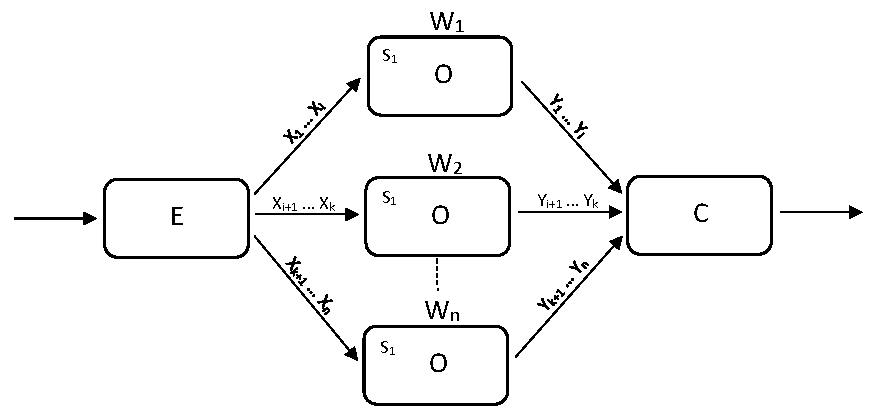
\includegraphics[width=1.0\textwidth]{Figures/DataParallelisme.pdf}
      \caption[Une repr\'esentation graphique du parall\'elisme de donn\'ees en \ppff.]{Une repr\'esentation graphique du parall\'elisme de donn\'ees. La m\^eme op\'eration~$O$ est ex\'ecut\'ee par les travailleurs $W_1, W_2,\ldots, W_n$ ($W$ pour \emph{$W$orker}). Le traitement associ\'e est repr\'esent\'e par le \emph{stage} $S_i$. Les \'el\'ements de donn\'ees sont r\'epartis entre les travailleurs par l'\'emetteur $E$ ($E$\emph{mitter}) puis les divers r\'esultats sont combin\'es par le collecteur $C$ ($C$\emph{ollector}).}
       \label{DataParallelisme.fig}
\end{figure}


L'impl\'ementation parall\`ele de ce mod\`ele peut \^etre
exprim\'ee sous la forme d'un ensemble de $n$ travailleurs $W_1, W_2,\ldots, W_n$ qui
appliquent une op\'eration $O$ sur les divers \'el\'ements~$X = \{x_1, \ldots, x_k\}$ apparaissant dans
le flux d'entr\'ee pour produire en sortie un ensemble d'\'el\'ements~$Y = \{y_1, \ldots, y_k\}$, o\`u $y_i = O(x_i)$.
%
Les divers \'el\'ements $x_i~(i=1, \ldots, k)$ sont r\'epartis entre
les travailleurs $W_j~(j=1, \ldots, n)$ d'une fa\c{c}on
ind\'etermin\'ee, qui d\'epend notamment de la vitesse de traitement
de chaque $x_i$.
%

La figure~\ref{DataParallelisme.fig} montre une repr\'esentation graphique du parall\'elisme de donn\'ees, o\`u la m\^eme op\'eration est ex\'ecut\'ee par les travailleurs $W_1, W_2,\ldots, W_n$. 

Il est possible de sp\'ecifier en param\`etre le nombre de travailleurs \`a utiliser pour l'ex\'ecution parall\`ele. Si ce param\`etre n'est pas sp\'ecifi\'e, un seul travailleur est activ\'e. Permettre ainsi d'augmenter le nombre de travailleurs fait en sorte qu'on peut augmenter le d\'ebit du traitement des donn\'ees si appropri\'e, c'est-\`a-dire, augmenter le nombre de donn\'ees qui peuvent \^etre trait\'ees en un temps donn\'e si le nombre de c\oe{}urs ou processeurs le permet.




\section{Stages}
\label{stages.sect}

\begin{figure}
\centering
     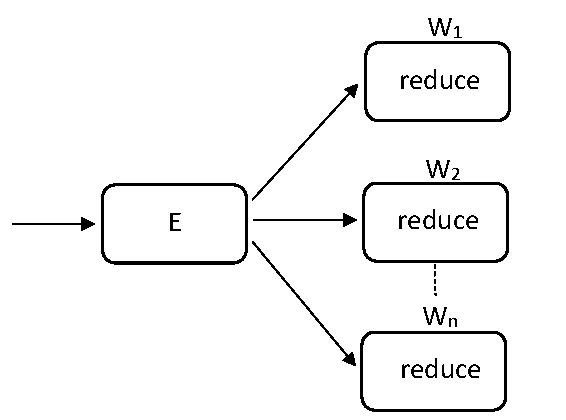
\includegraphics[width=0.7\textwidth]{Figures/StageDataParallel.pdf}
      \caption[Un exemple d'application de l'op\'eration \TT{reduce} sur diff\'erents sous-flux de donn\'ees.]{Un exemple d'application de l'op\'eration \TT{reduce} sur diff\'erents sous-flux de donn\'ees. C'est l'\emph{emitter} \TT{E} qui distribue les \'el\'ements $x_1, \ldots, x_k$ aux diff\'erents fils d'ex\'ecution $W_1, W_2, \ldots, W_n$ pour ainsi former les divers sous-flux de donn\'ees.}
       \label{StageDataParallel.fig}
\end{figure}



Le traitement en parall\`ele d'un flux de donn\'ees contribue \`a augmenter les performances du pipeline en utilisant les diff\'erents cœurs ou processeurs de la machine. Cependant, il existe une limitation lorsque le parall\'elisme de donn\'ees est appliqu\'e sur certaines op\'erations. Dans un flux, seules les op\'erations sans \'etat peuvent \^etre parall\'elis\'ees sans probl\`eme --- parce que sans interf\'erence. Par contre, quand il est n\'ecessaire de parall\'eliser une op\'eration avec \'etat --- par exemple, une r\'eduction avec un op\'erateur binaire ---, les choses deviennent un peu plus compliqu\'ees parce que le r\'esultat global du calcul est obtenu en combinant les r\'esultats produits pour les divers sous-flux de donn\'ees cr\'e\'es par la r\'epartition des \'el\'ements d'entr\'ee par l'\emph{Emitter}. Par exemple, la figure~\ref{StageDataParallel.fig} montre un exemple o\`u une op\'eration \TT{reduce} est appliqu\'ee en parall\`ele sur un flux d'\'el\'ements $x_1, \ldots, x_k$. Or, le r\'esultat global correct doit \^etre obtenu \emph{en combinant les r\'esultats du traitement de chacun des sous-flux} trait\'es dans chaque fil d'ex\'ecution ind\'ependant. Afin de permettre un tel traitement, nous avons introduit les \emph{stages}.

%Comme la plupart des traitements consistent en une combinaison d'op\'erations avec ou sans \'etat, un traitement parall\`ele ne peut pas \^etre effectu\'e. Une solution consiste alors \`a parall\'eliser les op\'erations sans \'etat et \`a utiliser un op\'eration \emph{Collector} pour fusionner les flux parall\`eles avant d'appliquer une op\'eration avec \'etat. Cette solution implique l'utilisation d'un autre cœur de la machine. De plus, le traitement pour les op\'erations avec \'etat est effectu\'e de fa\c{c}on s\'equentielle. Afin d'optimiser le traitement, nous avons introduit les \emph{stages}.

\begin{figure}
\centering
     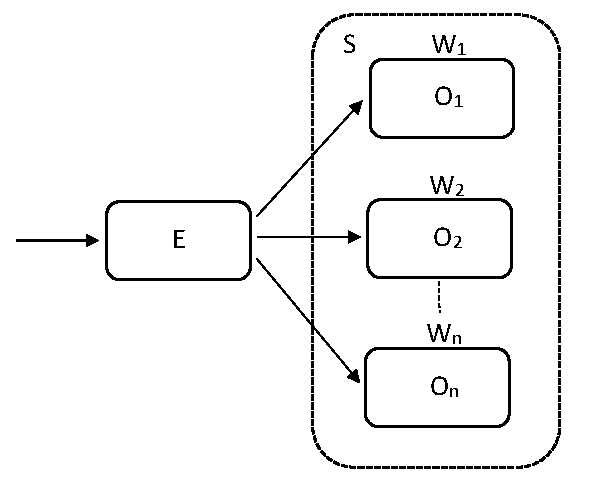
\includegraphics[width=0.7\textwidth]{Figures/Stages.pdf}
      \caption[Le groupement logique de $n$ op\'erations $O_1, O_2, \ldots, O_n$ dans un \TT{stage} S.]{Le groupement logique de $n$ op\'erations $O_1, O_2, \ldots, O_n$ dans un \TT{stage} S.  L'\emph{Emitter} E distribue les \'el\'ements $x_1, \ldots, x_k$ du flux aux diff\'erents fils d'ex\'ecution $W_1, W_2, \ldots, W_n$. Dans le cas d'une op\'eration avec \'etat (op\'eration finale), c'est l'objet \TT{Stage} qui combine ensemble les r\'esultats interm\'ediaires produits par les diff\'erents travailleurs.}
       \label{Stages.fig}
\end{figure}

\begin{figure}
\centering
     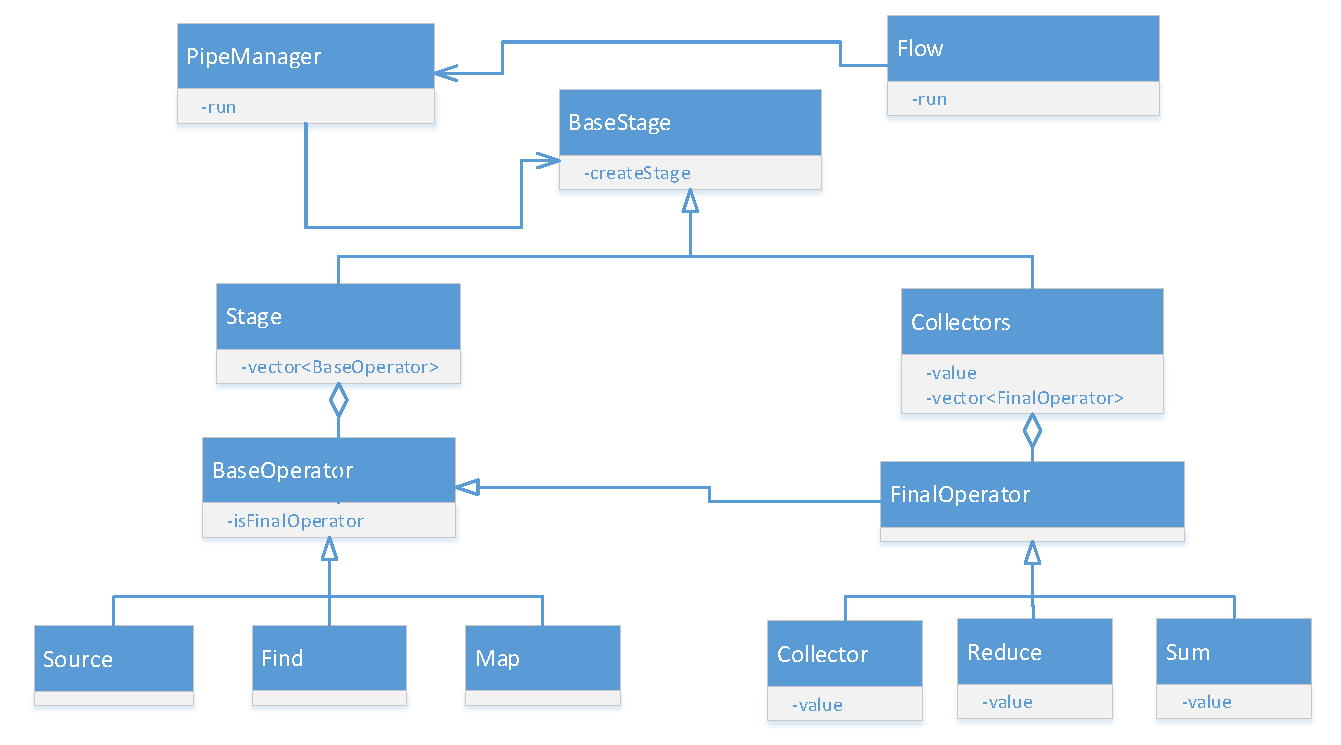
\includegraphics[width=1.0\textwidth]{Figures/StagesClassDiagramme.pdf}
      \caption{Le diagramme de classes pour la classe \texttt{Stage} et les classes associ\'ees.}
       \label{StagesClassDiagramme.fig}
\end{figure}



Un \emph{stage} repr\'esente le groupement logique d'une ou plusieurs op\'erations d'une \'etape dans la cha\^ine de traitement d'un pipeline. La figure~\ref{Stages.fig} montre plusieurs op\'erations finales group\'ees logiquement dans un \emph{stage}.  \`A noter que cette classe n'est pas visible \`a l'utilisateur. 

\begin{lstlisting}[
label={ImplementationOverridingOperator},
language=c++,
caption={[Le code source de l'op\'erateur \TT{operator+} de la classe \TT{CollectorOperator}.]Le code source de l'op\'erateur \TT{operator+} pour la classe \TT{CollectorOperator}.},
frame=single,
float]
template <typename T, typename TContainer>
class CollectorOperator: public FinalOperator {
public:
  CollectorOperator& operator+=(const CollectorOperator& other) {
    for (T elem: other.container) {
      container.push_back(elem);
    }

    return *this ;
  }	
  
private:
  TContainer container{};
};
\end{lstlisting}


\label{stages-finaux.sect}
%
Dans notre mise en \oe{}uvre, nous distinguons deux types de \emph{stages} : les \emph{stages} interm\'ediaires et les \emph{stages} finaux. Comme leur nom le sugg\`ere, les \emph{stages} interm\'ediaires groupent seulement les op\'erations sans \'etat et les \emph{stages} finaux groupent les op\'erations finales. La figure~\ref{StagesClassDiagramme.fig} montre la diagramme de classes pour la classe \TT{Stage} et les classes associ\'ees. Dans le cas du traitement parall\`ele, les \emph{stages} finaux ont pour r\^ole de r\'eduire l'\'etat d'op\'erations finales de chaque fil d'ex\'ecution selon l'op\'eration sp\'ecifi\'ee (cf.~Sect.~\ref{reducer.sect}). La valeur issue du flux repr\'esente le r\'esultat global du traitement du flux de donn\'ees.

Plus pr\'ecis\'ement, la valeur finale est obtenue en utilisant la
fonction \TT{operator+=} d\'efinie dans la classe \TT{BaseCollector}
(surcharg\'ee (\emph{overriden}) dans chaque \TT{Node}).
%
Lorsqu'un \TT{pipeline} termine son traitement, l'objet \TT{Stage}
associ\'e produit donc le r\'esultat final en appelant l'op\'erateur
\TT{operator+=} de chaque \TT{Node} associ\'e au \TT{Stage}. Le
listing~\ref{ImplementationOverridingOperator} montre
l'impl\'ementation de \TT{operator+=} dans l'un des op\'erateurs
finaux de \TT{PpFf}, \TT{CollectorOperator}. Dans ce cas, chaque
\'el\'ement du r\'esultat partiel (\TT{other.container}) produit par
chaque \emph{thread} est ajout\'e dans un conteneur~STL
\TT{container}, cr\'e\'e dans le constructeur de la classe \TT{Stage}.




\section{Impl\'ementation de \TT{PpFf} avec \TT{FastFlow} : un exemple}

\begin{lstlisting}[
label={listingExampleImplementationPpFf},
language=c++,
caption={[Le code source d'une petite application illustrant le fonctionnement de \ppff.]Le code source d'une petite application utilis\'ee pour d\'ecrire le fonctionnement de \ppff.},
frame=single,
float]
// Determine si une chaine est non-vide.
auto not_empty = [](std::string* s) {
  return s->size() > 0;
};
	
// Convertit les lettres Majuscules en minuscules.
auto to_lowercase = [](std::string* data) {
  std::string* result = new std::string;
  for (char c: *data) {
    if ('a' <= c && c <= 'z') {
   	  result->push_back(c);
   	} else if ('A' <= c && c <= 'Z') {
	  result->push_back(c-('Z'-'z')); // Majuscule -> minuscule.
   	} // else: on ignore le caractere.
  }
  return result;	
};

// Selectionne les chaines non-vides et les convertit en minuscules.
std::vector<std::string> result = 
  Flow
  ::source(path)
  .find<std::string>(not_empty)
  .parallel(2)
  .map<std::string, std::string>(to_lowercase)
  .collect<std::string, std::vector>();
\end{lstlisting}



Cette section d\'ecrit le mod\`ele d'ex\'ecution de \ppff\ \`a l'aide du code source d'une petite application. Illustr\'ee dans le listing~\ref{listingExampleImplementationPpFf}, l'application est compos\'ee des \'el\'ements suivants :
\begin{itemize}
	\item  \TT{source}, qui g\'en\`ere un flux s\'equentiel de lignes \`a partir d'un fichier --- le fichier est identifi\'e par le param\`etre \TT{path} fourni en argument;

	\item  \TT{find}, qui s\'electionne dans le flux d'entr\'ee les mots qui ne sont pas vides (\texttt{not\_empty});

	\item \TT{parallel}, qui indique que les op\'erations subs\'equentes doivent \^etre ex\'ecut\'ees en parall\`ele, ici, avec deux (2) \emph{threads};
	
	\item \TT{map}, qui transforme les lettres majuscules du mot en lettres minuscules (\texttt{to\_lowercase});
	
	\item Finalement, \TT{collect}, qui combine tous les \'el\'ements obtenus dans un conteneur de type \TT{vector}.
\end{itemize}

\begin{figure}
\centering
     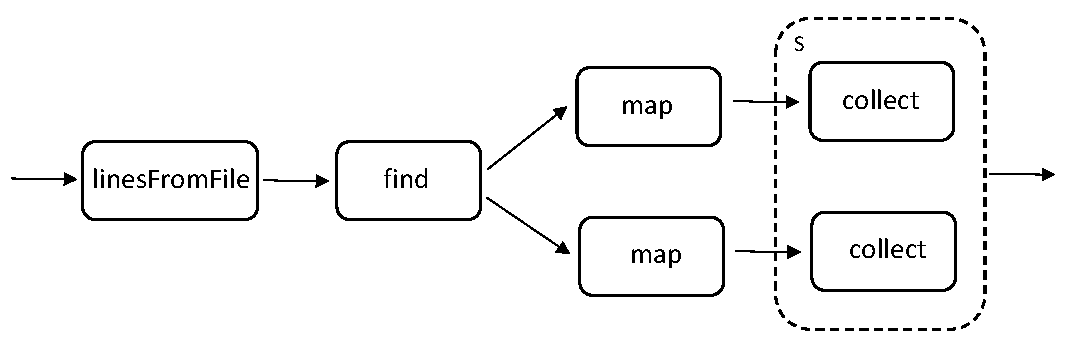
\includegraphics[width=\textwidth]{Figures/ExempleRuntimeExecution.pdf}
      \caption[Une repr\'esentation graphique d'un \TT{pipeline} compos\'e de quatre op\'erations.]{Une repr\'esentation graphique d'un \TT{pipeline} compos\'e de quatre op\'erations ex\'ecut\'ees en parall\`ele. Du parall\'elisme de flux est appliqu\'e sur les deux premi\`eres op\'erations et du parall\'elisme de donn\'ees est appliqu\'e sur les derni\`eres op\'erations. Le~\texttt{S}~sur la boite pointill\'ee \`a droite indique un \emph{Stage}.}
       \label{ExempleRuntimeExecution.fig}
\end{figure}


La figure~\ref{ExempleRuntimeExecution.fig} montre la repr\'esentation graphique d'un \TT{Pipeline} compos\'e des op\'erations d\'ecrites dans le listing~\ref{listingExampleImplementationPpFf}.
 

La classe \TT{Pipeline} de l'API repr\'esente l'entit\'e principale de l'application. \`A l'ex\'ecution, un \TT{Pipeline} correspond \`a une classe \TT{ff\_pipeline} de \TT{FastFlow}. Un \TT{Pipeline} est compos\'e de plusieurs nœuds de type \TT{ff\_node} ou \TT{ff\_farm}. 

Dans un \TT{Pipeline}, la premi\`ere op\'eration est toujours une op\'eration d'entr\'ee, laquelle est impl\'ement\'ee sous forme d'un \TT{ff\_node}. Dans notre exemple, \TT{source} renvoie un flux s\'equentiel de lignes \`a partir d'un fichier. De plus, l'op\'eration d'entr\'ee a aussi la t\^ache d'envoyer un signal \TT{EOS} (\emph{\texttt{E}nd \texttt{O}f \texttt{S}tream}) lorsque la g\'en\'eration du flux d'entr\'ee est termin\'ee~: \TT{EOS} indique aux nœuds \TT{ff\_node}s de \TT{FastFlow} de terminer leur ex\'ecution apr\`es la r\'eception de celui-ci.

La classe repr\'esentant chaque nœud dans un \TT{Pipeline} contient les informations concernant son r\^ole dans la chaine de traitement. Par exemple, l'op\'eration \TT{find} du listing~\ref{listingExampleImplementationPpFf} a pour r\^ole de s\'electionner dans le flux seulement les mots qui ne sont pas vides. Ce r\^ole est d\'efini par l'utilisateur \`a la cr\'eation du \TT{Pipeline}, en fournissant une fonction ou une expression lambda \`a \TT{find}.


Les divers op\'erations d'un \TT{Pipeline} sont toujours ex\'ecut\'ees en parall\`ele~: dans \TT{FastFlow}, chaque \TT{ff\_node} est associ\'e \`a un \emph{thread} ind\'ependant, donc le mod\`ele de parall\'elisme de flux est appliqu\'e par d\'efaut. 

En outre, lorsqu'un appel \`a la m\'ethode \TT{parallel} est ajout\'e dans la chaine du traitement d'un \TT{Pipeline}, les op\'erations subs\'equentes sont ex\'ecut\'ees en parall\`ele, et ce en utilisant du parall\'elisme de donn\'ees. Dans l'exemple du listing~\ref{listingExampleImplementationPpFf}, les deux premi\`eres op\'erations sont ex\'ecut\'ees en parall\`ele, avec du parall\'elisme de flux, alors que du parall\'elisme de flux et du parall\'elisme de donn\'ees sont aussi utilis\'es pour les op\'erations suivantes (apr\`es \TT{parallel}). 

Dans l'impl\'ementation de \TT{PpFf}, le parall\'elisme de donn\'ees est mis en œuvre avec la classe \TT{ff\_farm} de \TT{FastFlow}. La cr\'eation du flux de traitement en utilisant le mod\`ele de parall\'elisme de donn\'ees est simple. Lorsque la m\'ethode \TT{parallel()} est invoqu\'ee, une instance de la classe \TT{ff\_farm} est ajout\'ee dans le \TT{Pipeline}. Pour chaque \emph{worker} de \TT{ff\_farm}, un nouveau \TT{ff\_pipeline} est cr\'e\'e. Les op\'erations ajout\'ees dans la chaine du traitement  sont ajout\'ees comme nœuds dans les nouveaux \TT{ff\_pipeline} cr\'e\'es. Par exemple, les op\'erations \TT{map} et \TT{collect} du listing~\ref{listingExampleImplementationPpFf} sont ajout\'ees dans le \TT{pipeline} de chaque \TT{worker} de \TT{ff\_farm}. 


\begin{figure}
\centering
     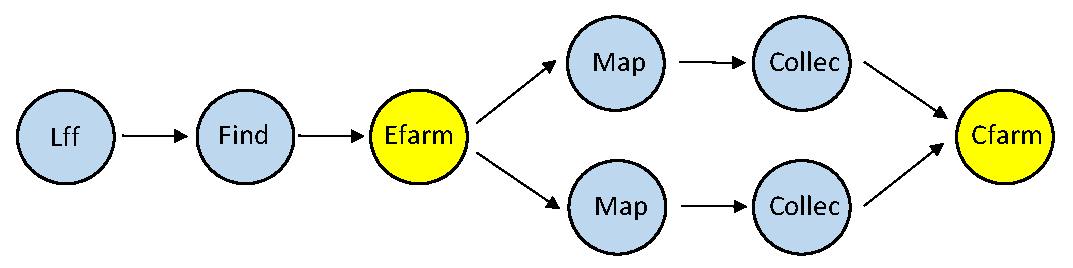
\includegraphics[width=\textwidth]{Figures/ExempleRuntimeExecutionFF.pdf}
      \caption[Une repr\'esentation graphique du listing~\ref{listingExampleImplementationPpFf} en \TT{FastFlow}.]{Une repr\'esentation graphique du listing~\ref{listingExampleImplementationPpFf} en \TT{FastFlow}. Les cercles bleus repr\'esentent les op\'erations sp\'ecifi\'ees par l'utilisateur : \TT{linesFromFile} (\texttt{Lff}), \TT{find} (\texttt{Find}), les deux \TT{map} (\texttt{Map}) et les deux \TT{collector} (\texttt{Collec}). Les cercles en jaunes repr\'esentent l'\emph{Emitter} et le \emph{Collector} du \TT{ff\_farm}.}
       \label{ExempleRuntimeExecutionFF.fig}
\end{figure}


La figure~\ref{ExempleRuntimeExecutionFF.fig} montre la repr\'esentation graphique du pipeline \TT{FastFlow} qui met en \oe{}uvre le pipeline \PpFf\ de la figure~\ref{ExempleRuntimeExecution.fig}. Chaque cercle est une classe de type \TT{ff\_node}. Les cercles en bleu repr\'esentent les op\'erations sp\'ecifi\'ees par l'utilisateur : \TT{linesFromFile} (Lff), \TT{find} (Find), les deux \TT{map} (Map) et les deux \TT{collector} (Collec). Les cercles en jaunes repr\'esentent l'\emph{Emitter} et le \emph{Collector} de l'objet \TT{ff\_farm}. 


L'ex\'ecution parall\`ele d'un flux est r\'ealis\'ee par l'ex\'ecution de la m\'ethode \TT{run\_and\_wait\_end()} de la classe \TT{ff\_pipeline} de \TT{FastFlow}. Chaque \TT{ff\_node} de \TT{ff\_pipeline} est une instance de la classe C++ \TT{ff\_node} qui ex\'ecute une boucle de traitement qui va comme suit:
\begin{itemize}
	\item obtient du canal d'entr\'ee (via un pointeur) un \'el\'ement \`a traiter;
	\item ex\'ecute le code sur l'\'el\'ement, code indiqu\'e dans la m\'ethode \TT{svc()};
	\item \'emet dans le canal de sortie (via un pointeur)  l'\'el\'ement produit.
\end{itemize}



Les nœuds d'un pipeline sont ex\'ecut\'es jusqu'\`a ce qu'ils re\c coivent le signal \TT{EOS}. \`A ce moment, tous les nœuds sont d\'etruits. Dans le cas de noeuds multiples associ\'es \`a du parall\'elisme de donn\'ees, le r\'esultat global de l'op\'eration est obtenu en combinant les r\'esultats des sous-flux produits par les divers fils d'ex\'ecution. Par exemple, chaque op\'eration \TT{collect} repr\'esent\'ee dans la figure~\ref{ExempleRuntimeExecution.fig} collecte le r\'esultat du traitement de chacun des sous-flux trait\'es dans un fil d'ex\'ecution ind\'ependant. Le r\'esultat global est obtenu via la classe \TT{Stage} qui combine ces r\'esultats interm\'ediaires, tel qu'expliqu\'e \`a la section~\ref{stages-finaux.sect}


\section{Quelques donn\'ees sur la mise en \oe{}uvre}

\GT{Dans un des rapports, il était indiqué <<Les métriques de code
présentées (nombre de lignes, etc.) ne sont pas pertinentes si elles
ne sont pas discutées.>> Or, pour l'instant, je ne sais pas trop quel
genre de discussion tu pourrais/devrais faire. Une possibilité si on
ne trouve pas~: simplement mettre cette section dans une annexe?}


\begin{center}
\footnotesize
\begin{longtable}{|l|r|r|r|r|r|r|}
\caption{Donn\'ees sur la mise en \oe uvre~: les modules et le fichier \TT{Flow.hpp}.\label{statistiquesPpFf.tab}}\\
\hline

& \multicolumn{5} {c|}{\textbf{Module}}&\\
\hline
& \textbf{pipeline} & \textbf{operators} & \textbf{stages} & \textbf{utilities} & \textbf{collections} & \textbf{Flow.hpp}\\
\hline
%\endhead
\hline
	\textbf{Nombre de fichiers} &	
	5 &
	26 &
	6 &
	3 &
	1 &
    1
    \\
\hline
	\textbf{Nombre de lignes} &
	297 &
	1225 &
	201 &
	42 &
	124 &
    345
    \\                 
\hline    
\end{longtable}
\normalsize
\end{center} 



Cette section donne un aper\c {c}u de l'envergure du projet r\'ealis\'e. \TT{PpFf} est divis\'e en plusieurs modules. Le tableau~\ref{statistiquesPpFf.tab} pr\'esente quelques donn\'ees sur la mise en \oe uvre~: nombre de fichiers et nombre de lignes de code dans chaque module. Il faut noter que les lignes blanches et les lignes de commentaires ont \'et\'e prises en compte lors du calcul des nombres de lignes de code.


\begin{itemize}
\item Le module \TT{pipeline} est le c\oe ur du traitement des flux~: il g\`ere la cr\'eation des \TT{pipeline}s, le traitement en parall\`ele et la communication entre les n\oe uds composant un \TT{pipeline}~; il g\`ere aussi la communication entre \TT{FastFlow} et \TT{PpFf}.

\item Le plus grand module du projet est  \TT{operators}. Totalisant 1225 de lignes de code, ce module d\'efinit la logique de traitement de chacune des op\'erations de l'\TT{API}. 

\item Le module \TT{stages} g\`ere le groupement logique d'une ou plusieurs op\'erations d'une \'etape dans la cha\^ine de traitement d'un \TT{pipeline}. 

\item Tout projet a besoin d'objets et de fonctionnalit\'es qui sont partag\'es par d'autres modules. Dans \TT{PpFf}, ces objets sont regroup\'es dans le module \TT{utilities}, le plus petit module de l'\TT{API}.

\item Le module \TT{collections} est le dernier module dans le traitement de flux. Il g\`ere la collecte des \'el\'ements du flux dans un conteneur apr\`es leur traitement.  
 
\item Les m\'ethodes permettant \`a l'utilisateur de manipuler des flux de donn\'ees sont regroup\'ees dans le fichier \TT{Flow.hpp}. Avec 345 lignes de code, ce fichier est le point d'entr\'ee de l'API. Plus pr\'ecis\'ement, c'est l'interface utilisateur de \TT{PpFf}. 

\end{itemize}

\begin{center}
\footnotesize
\begin{longtable}{|r|r|r|}
\caption{Donn\'ees sur les tests unitaires.\label{statistiquesUnitTest.tab}}\\
\hline

\textbf{Nb.\ de m\'ethodes de l'API} & \textbf{Nb.\ de cas de tests} & \textbf{Nb.\ d'assertions \'evalu\'ees}\\
\hline
%\endhead
\hline
	21 &
	123 &
	13~895
    \\                   
\hline    
\end{longtable}
\normalsize
\end{center} 

Chaque fonctionnalit\'e d\'efinie dans l'interface de \ppff\ est test\'ee avec des tests unitaires. L'outil utilis\'e est \TT{catch},%
%
\footnote{\url{https://github.com/catchorg/Catch2}}
%
un cadre de tests unitaires en \TT{C++} qui utilise un unique fichier
d'en-t\^ete.
%
\TT{catch} peut \^etre utilis\'e avec une approche de tests TDD
(\emph{Test-Driven Development}) avec assertions, 
ou avec une approche BDD (\emph{Behavior Driven Development}), avec \TT{Given--When--Then}.




Le tableau~\ref{statistiquesUnitTest.tab} pr\'esente quelques donn\'ees sur les tests cr\'e\'es.

Chaque m\'ethode de l'API a son propre fichier de test contenant plusieurs cas de test. Au total, les 21 m\'ethodes expos\'ees \`a l'utilisateur sont test\'ees avec 123 cas de tests. Plusieurs assertions sont g\'en\'er\'ees pour chaque cas de test. Au nombre de 13~895, le nombre d'assertions \'evalu\'ees est beaucoup plus grand que le nombre de cas de tests, et ce \`a cause de la fa\c{c}on dont sont test\'ees les structures de donn\'ees --- par ex., chaque \'el\'ement d'un tableau g\'en\'ere l'\'evaluation d'une assertion.

